\section{Estrategia de resolución}% mediante acoplamiento de códigos}

\subsection{Paradigma maestro-esclavo}

\begin{frame}
{Estrategia de resolución mediante acoplamiento de códigos}
{Paradigma maestro-esclavo}
%~ 
% ~ \begin{figure}
\centering
\begin{tikzpicture}[
  scale=0.7, every node/.style={scale=0.7},
	block1/.style={
	draw,
	fill=white,
	rectangle, 
	%~ minimum width={width("Proceso $N_m$")+2pt},
	%~ minimum height={15pt},
	font=\small},
	block2/.style={
	draw,
	%~ fill=white,
	rectangle,
  fill=blue!20,
  text centered, 
  rounded corners,
	%~ minimum width={width("Esclavo N")+2pt},
	%~ minimum height={15pt},
	font=\large},
	connector/.style={
	-o,
	line width=0.3mm
	},
  arrow1/.style={
  -{Latex[length=3mm, width=1mm]}
  },
  arrow2/.style={
  {Latex[length=3mm, width=1mm]}-{Latex[length=3mm, width=1mm]}
  }]

	% Dummy
	\node at (0,10em)             (dummy) {}; % blank space

	% Master
	\node [draw,fill=blue!20,text centered,rounded corners] at (0,8em)             (master) {\textbf{Maestro}};
	\node [block2] at (0,8em)             (master) {\textbf{Maestro}};
	\node [block1, below=1em of master]   (masterp1) {...};
	\node [block1, left=1em of masterp1]  (masterp0) {Proceso $0_m$};	
	\node [block1, right=1em of masterp1] (masterpN) {Proceso $N_m$};

	% Slave 1
	\node [block2] at (-6.5,0em)    		(slave1) {\textbf{Esclavo 1}};
	\node [block1, below=1em of slave1] (s1p0) 	 {Proceso $0_1$};
	\node [block1, below=1em of s1p0]   (s1p1) 	 {...};
	\node [block1, below=1em of s1p1] 	(s1pN) 	 {Proceso $N_1$};
	%~ 
	% Slave 2
	\node [block2] at (-3.5,-4em)    		(slave2) {\textbf{Esclavo 2}};
	\node [block1, below=1em of slave2] (s2p0) 	 {Proceso $0_2$};
	\node [block1, below=1em of s2p0]   (s2p1) 	 {...};
	\node [block1, below=1em of s2p1] 	(s2pN) 	 {Proceso $N_2$};
	
	% Slave 3
	\node [block2] at (0,0em)      		  (slave3) {\textbf{Esclavo 3}};
	\node [block1, below=1em of slave3] (s3p0) 	 {Proceso $0_3$};
	\node [block1, below=1em of s3p0]   (s3p1) 	 {...};
	\node [block1, below=1em of s3p1] 	(s3pN) 	 {Proceso $N_3$};
	
	% Slave 4
	\node [block2] at (3.5,-4em)   		  (slave4) {\textbf{Esclavo $i$}};
	\node [block1, below=1em of slave4] (s4p0) 	 {Proceso $0_i$};
	\node [block1, below=1em of s4p0]   (s4p1) 	 {...};
	\node [block1, below=1em of s4p1] 	(s4pN) 	 {Proceso $N_i$};
	
	% Slave N
	\node [block2] at (6.5,0em)    		  (slave5) {\textbf{Esclavo N}};
	\node [block1, below=1em of slave5] (s5p0) 	 {Proceso $0_N$};

	% Processes
	\draw[connector] (master.south) -- ($(masterp0.north)+(0,0.2em)$);
	\draw[connector] (master.south) -- ($(masterp1.north)+(0,0em)$);
	\draw[connector] (master.south) -- ($(masterpN.north)+(0,0.2em)$);

	\draw[connector] (slave1.west) -- ++(-1em,0) |- (s1p0.west);
	\draw[connector] (slave1.west) -- ++(-1em,0) |- (s1p1.west);
	\draw[connector] (slave1.west) -- ++(-1em,0) |- (s1pN.west);

	\draw[connector] (slave2.west) -- ++(-1em,0) |- (s2p0.west);
	\draw[connector] (slave2.west) -- ++(-1em,0) |- (s2p1.west);
	\draw[connector] (slave2.west) -- ++(-1em,0) |- (s2pN.west);

	\draw[connector] (slave3.west) -- ++(-1em,0) |- (s3p0.west);
	\draw[connector] (slave3.west) -- ++(-1em,0) |- (s3p1.west);
	\draw[connector] (slave3.west) -- ++(-1em,0) |- (s3pN.west);

	\draw[connector] (slave4.west) -- ++(-1em,0) |- (s4p0.west);
	\draw[connector] (slave4.west) -- ++(-1em,0) |- (s4p1.west);
	\draw[connector] (slave4.west) -- ++(-1em,0) |- (s4pN.west);

	\draw[connector] (slave5.west) -- ++(-1em,0) |- (s5p0.west);


	% Comunicators
	\draw[arrow2] ($(masterp0.south)-(1em,0)$) to[out=-90, in=15, distance=2em] node [midway, sloped, anchor=center, above]{\textit{MPI}} (s1p0.east);

	\draw[arrow2] ($(masterp0.south)+(0em,0)$) to[out=-90, in=35, distance=3em] node [midway, rotate=90, anchor=center, above]{\textit{MPI}} (s2p0.east);

	\draw[arrow1] ($(masterp0.south)+(1em,0)$) to[out=-90, in=105, distance=2em] node [midway, sloped, anchor=center, above]{\textit{I/O}} (slave3.north);

	\draw[arrow1] (masterp1.south) to[out=-90, in=105, distance=2em] node [midway, sloped, anchor=center, above]{\textit{I/O}} (slave4.north);

	\draw[arrow1] (masterpN.south) to[out=-90, in=105, distance=2em] node [midway, sloped, anchor=center, above]{\textit{I/O}} (slave5.north);

\end{tikzpicture}
%~ \end{figure}

\end{frame}


% \subsection{Modelos de comunicación}

% \begin{frame}
% {Estrategia de resolución mediante acoplamiento de códigos}
% {Modelos de comunicación}

% \begin{itemize}
% \item <1-> Paso de mensajes: este modelo es implementado para comunicar procesos de programas en los cuales es posible modificar sus códigos fuente.
%   \begin{itemize}
%   \item Programas ejecutados en forma independiente y conectados
%   \item Programas ejecutados en simultáneo como argumentos de $mpirun$
%   \end{itemize}
% \item <2-> Escritura de archivos de entrada y lectura de archivos de salida: este modelo es implementado para comunicar procesos de programas en los cuales NO es posible modificar sus códigos fuente.
% \end{itemize}

% \end{frame}


% \subsection{Arquitectura de acoplamiento montada en códigos esclavos comunicados por paso de mensajes}
% \subsection{Paradigma maestro esclavo}

\begin{frame}
{Estrategia de resolución mediante acoplamiento de códigos}
{Paradigma maestro-esclavo}
% {Arquitectura de acoplamiento montada en códigos esclavos comunicados por paso de mensajes}

\begin{figure}
\centering{}
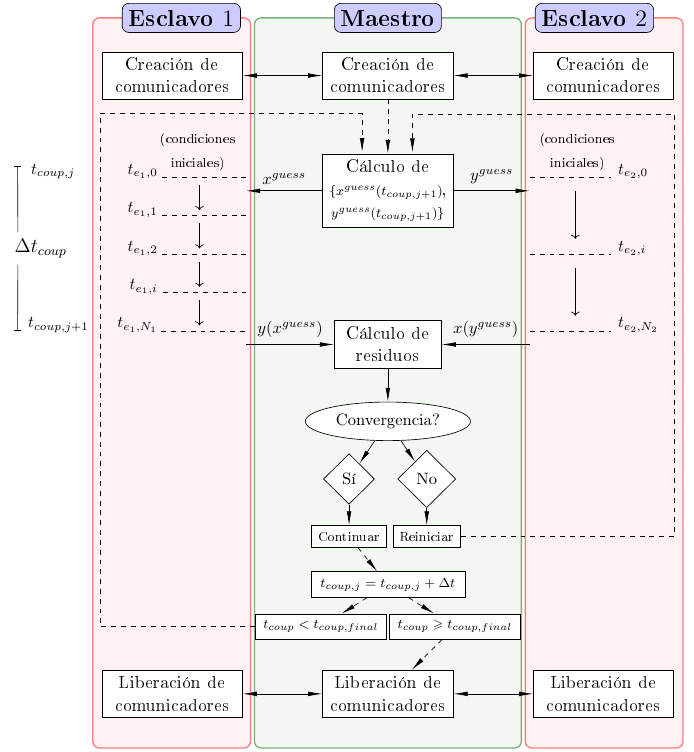
\includegraphics[scale=0.27]{esquema-acoplamiento.png}
\end{figure}


\end{frame}

% \subsection{Códigos maestro utilizados}

% \begin{frame}
% {Estrategia de resolución mediante acoplamiento de códigos}
% {Códigos maestro utilizados}

% \begin{itemize}
% \item \textbf{Coupling} \cite{coup-0d3d} \cite{coup-black} \cite{coup-hyd}
%   \begin{itemize}
%   \item <1-> Modelos de comunicación por paso de mensajes entre programas ejecutados de manera independiente
%   \item <2-> Cada interfaz de acople tiene $N$ pares de variables incógnitas
%   \item <3-> Métodos de resolución explícitos e implícitos implementados
%   \end{itemize}
% \end{itemize}

% \end{frame}

% \begin{frame}
% {Estrategia de resolución mediante acoplamiento de códigos}
% {Códigos maestro utilizados}

% \begin{itemize}
% \item \textbf{Newton} (desarrollado durante la maestría)
%   \begin{itemize}
%   \item <1-> Modelos de comunicación por paso de mensajes entre programas ejecutados de manera independiente o simultánea
%   \item <2-> Modelos de comunicación por manejo de archivos
%   \item <3-> Cada subsistema tiene $N$ incógnitas (extensión a acoplamientos genéricos)
%   \item <4-> Métodos de resolución explícitos e implícitos implementados
%   \item <5-> Mapeos de variables de entrada y salida ($\alpha-\beta$ y $\gamma-\delta$)
%   \end{itemize}
% \end{itemize}

% %~ \begin{figure}
% \centering{}
% \visible <5>{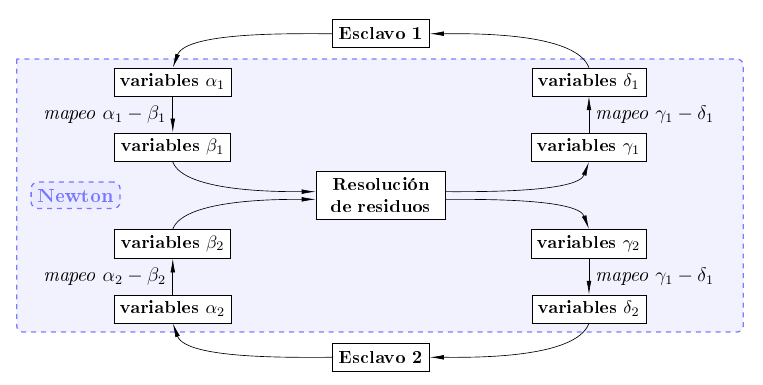
\includegraphics[scale=0.4]{abgd.png}}
% %~ \end{figure}

% \end{frame}
